\documentclass{article}
\usepackage[utf8]{inputenc}
\usepackage{url}
\usepackage{graphicx}
\usepackage{hyperref}
\usepackage{amsmath}
\graphicspath{ {./} }


\title{Automatisation du prétraitement de photographies de portraits de mandrills}
\author{Maxime Boucher}
\date{Compte rendu 10}

\begin{document}

\maketitle

Après avoir créer la base de données et réécrit les méta-données sous un format plus robuste, j'ai ajouté l'âge des mandrills dans celle-ci en calculant leur âge, en jours, à partir de la date de la prise de photo et de leur date de naissance, lorsque celle-ci est connue.

\begin{center}
    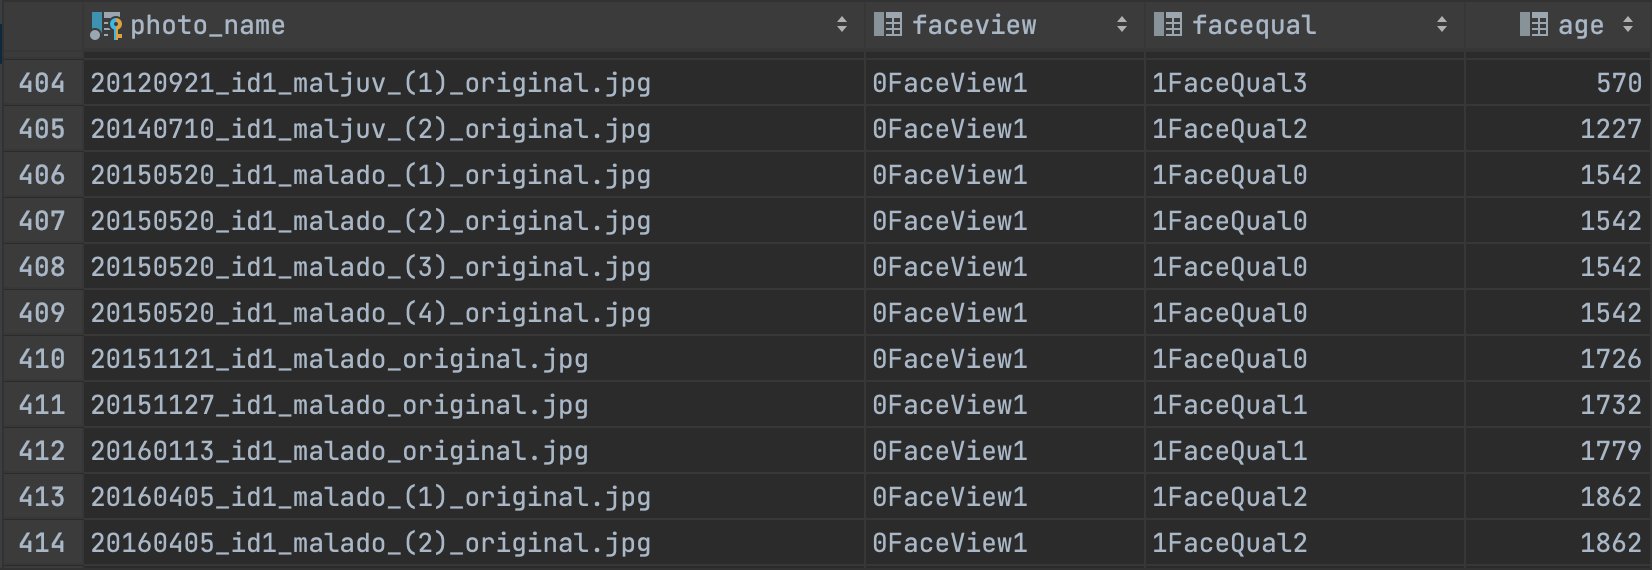
\includegraphics[width=345]{imgs/qualité/cr10/age.png}
\end{center}

Ensuite, pour finaliser mes résultats sur la prédiction de la qualité ainsi que la prédiction de la posture (face, profil), j'ai lancé une recherche "gridsearch" qui permet de scanner tous les combinaisons de paramètres différents que l'on veut optimiser.

Voici un exemple de fonctionnement simple ci-dessous, en faisant varier le learning rate et batch size.
\begin{center}
    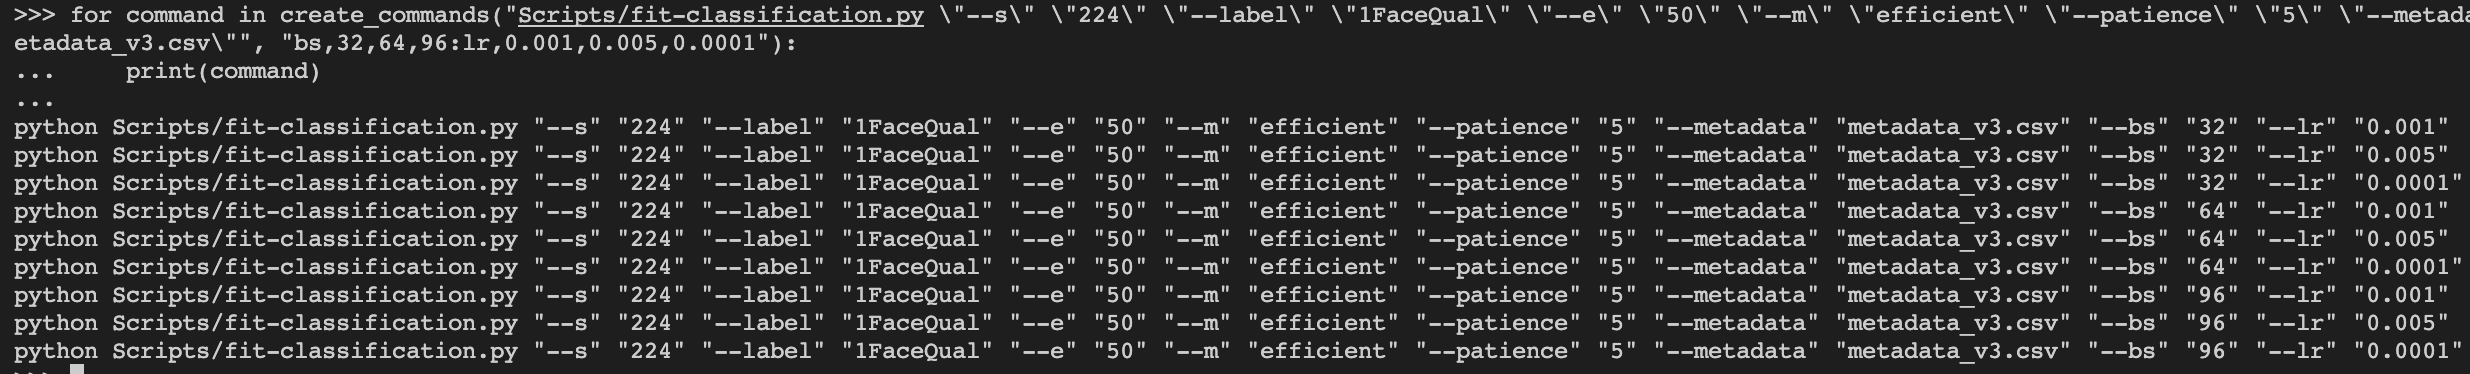
\includegraphics[width=345]{imgs/qualité/cr10/gridsearch2.png}
\end{center}


\end{document}
